\documentclass[11pt]{article}
\usepackage{empheq}
\usepackage[most]{tcolorbox}
\usepackage{wasysym}
\usepackage{hyperref}

\providecommand{\tightlist}{%
  \setlength{\itemsep}{0pt}\setlength{\parskip}{0pt}}
  
%Gummi|065|=)
\title{\textbf{ES 229 - Problem Set 5}}
\author{Benjamin Sanchez Lengeling}
\date{\today}
\usepackage{graphicx}
\begin{document}

\definecolor{harvardcrimson}{rgb}{0.79, 0.0, 0.09}
\definecolor{ghostwhite}{rgb}{0.97, 0.97, 1.0}
\newtcbox{\mymath}[1][]{%
    nobeforeafter, math upper, tcbox raise base,
    enhanced, colframe=black!30!harvardcrimson,
    colback=harvardcrimson!10, boxrule=1pt,#1}
    
\maketitle
\setcounter{section}{0}
\section{Preliminaries}
\subsection{Code repo}
All code for figures and calculations, along with data for reproduction of results can be found as a github repo at \url{}.

In particular the file \url{}, is an ipython notebook that shows the code step by step.

\subsection{Wedges}

Using historical data from 1990 to 2014 we can adjust a linear trend to make predictions of how many wedges we might need in 2064 (50 years from the last data point, 2014). Data is obtained from \url{http://cdiac.ornl.gov/trends/emis/tre_glob_2014.html}, which are measurements for Carbon emissions in billions of metric tons. The Triangle of stability is the composition of all wedges.

\begin{figure}[htp]
\centering
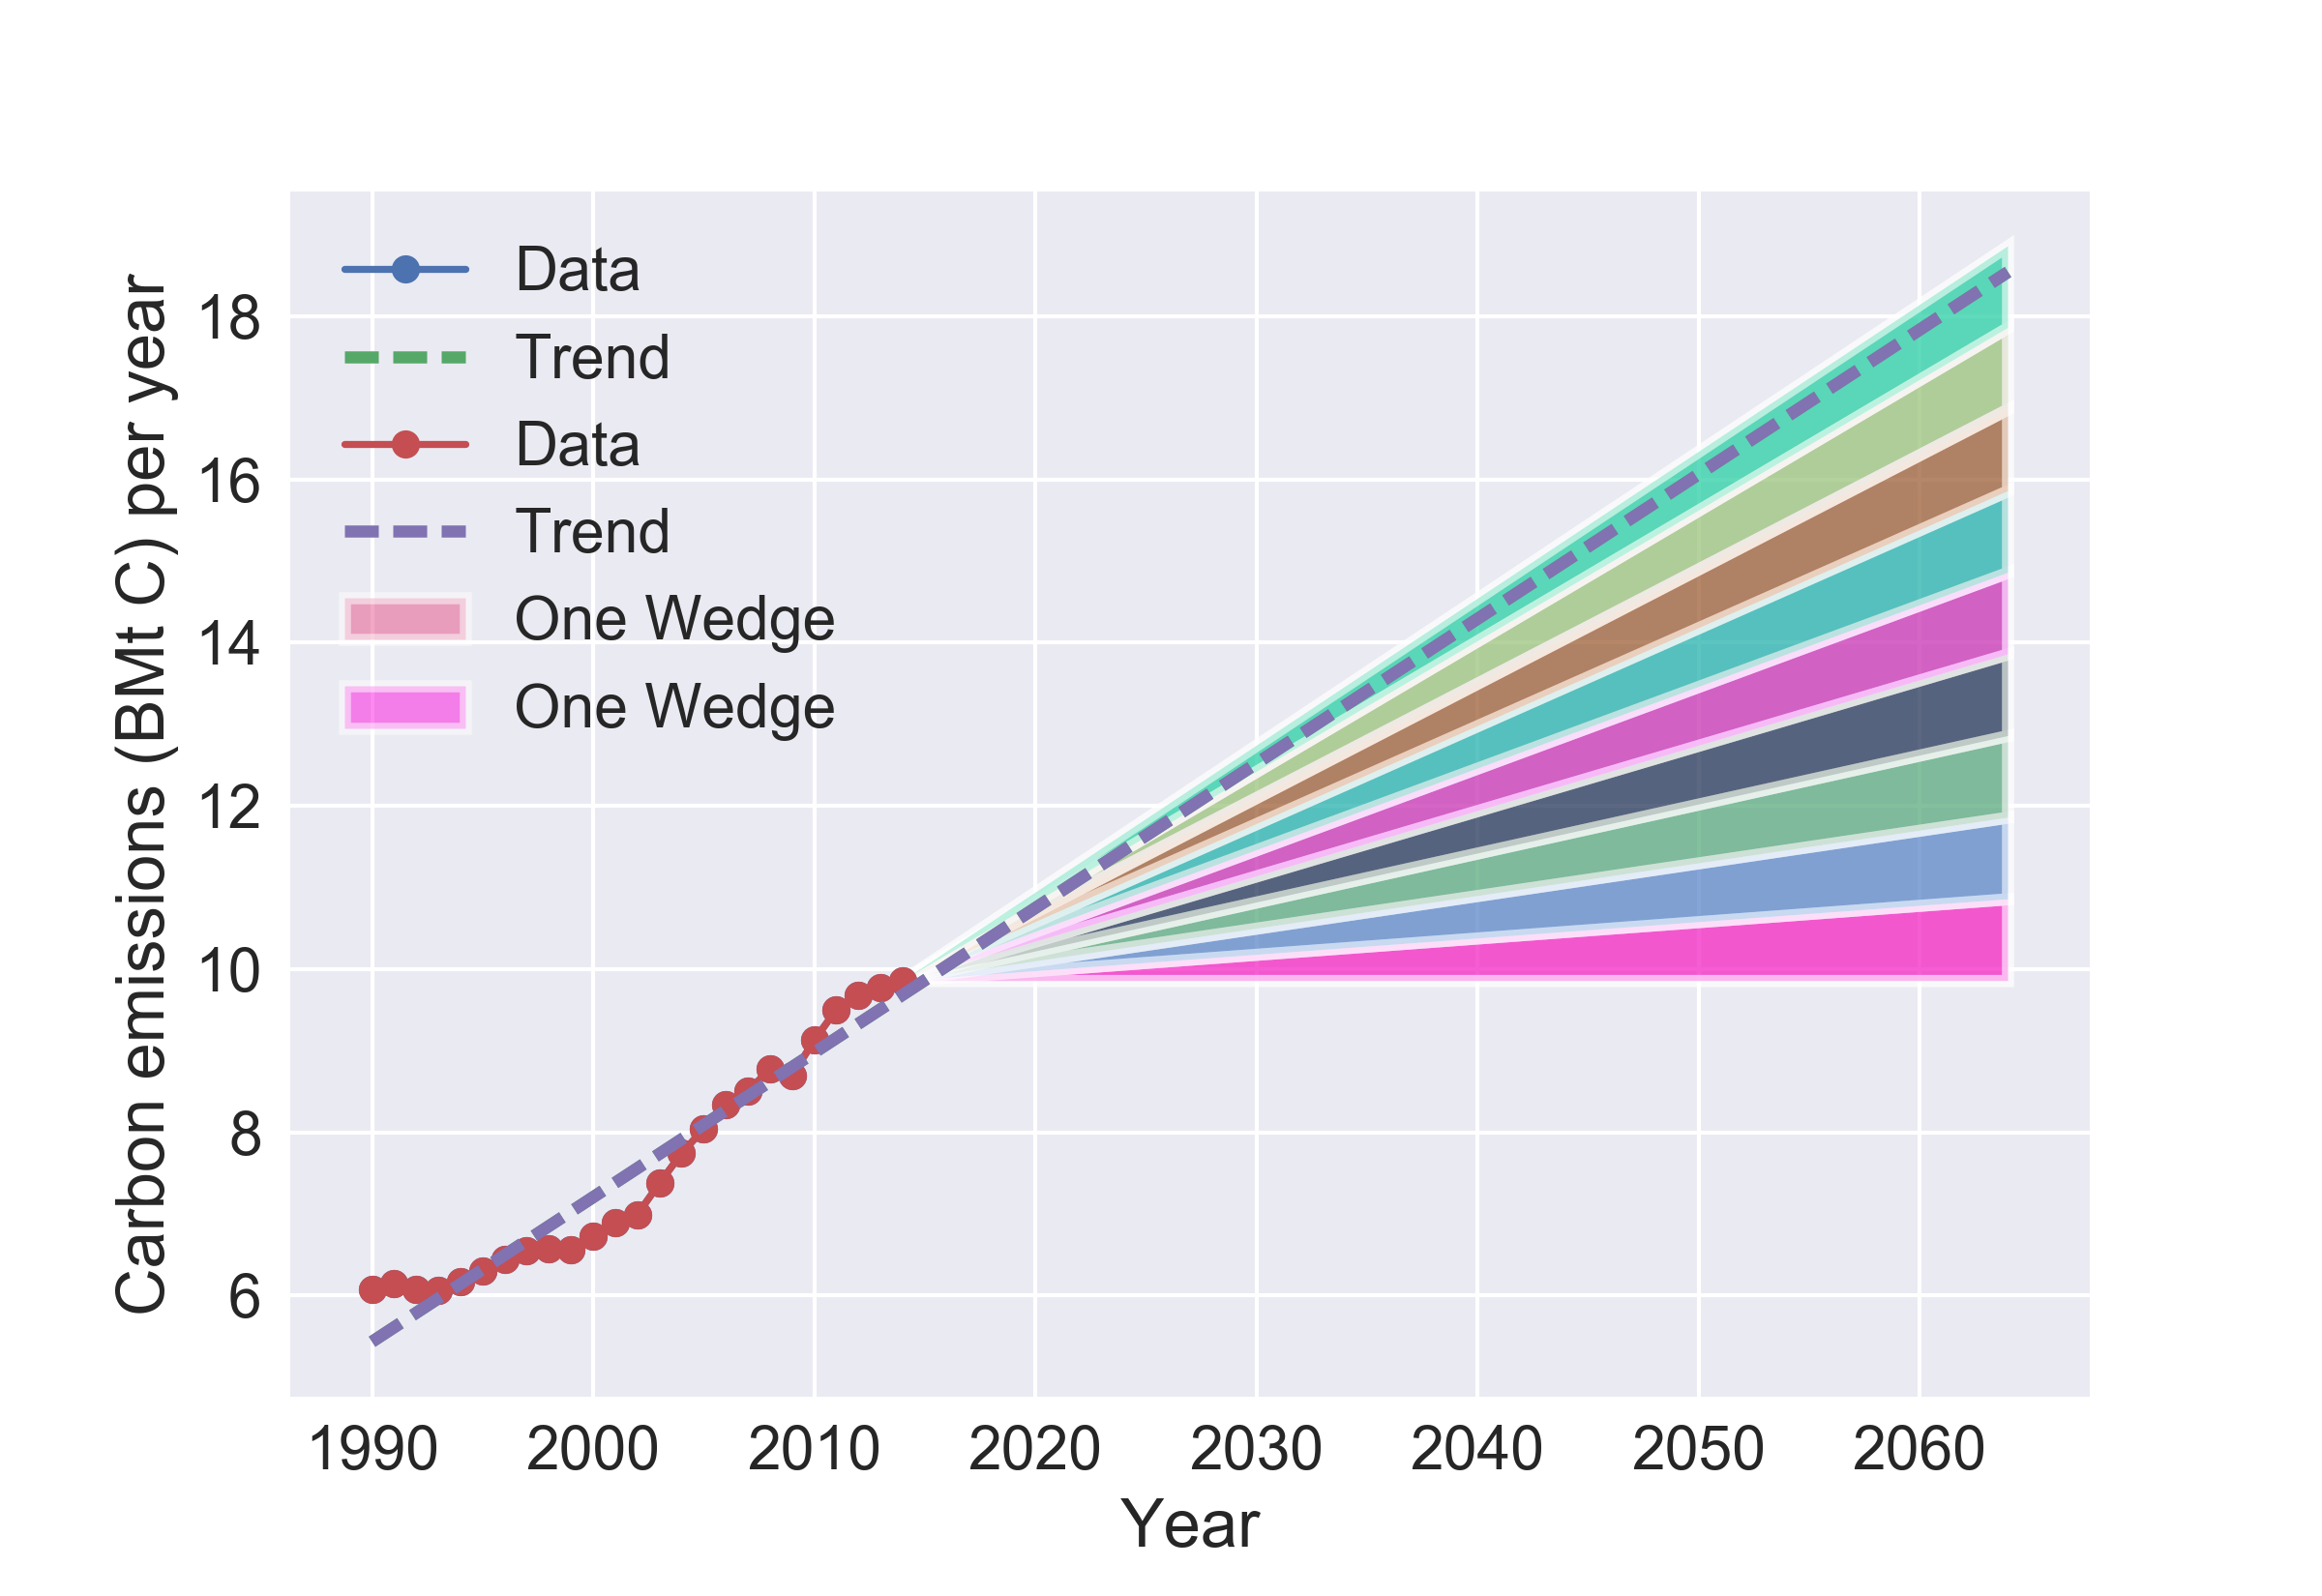
\includegraphics[scale=0.5]{wedge_calculator/c_emissions.png}
\caption{Projected carbon emissions up to 2064 based on a linear trend with data from 1990 to 2014.}
\label{}
\end{figure}

From this trend we predict the 2064 Carbon emission will be at 18.540 BMt C per year, which when compared to 2014 is a differential of 8.685 BMt C per year. If each wedge is one BMt C per year, then we have around 8 wedges and a medium size wedgie to curve our behavior.

\subsection{Gross World Product (GWP)}
Acoording to the World Bank (\url{http://databank.worldbank.org/data/download/GDP.pdf} and \url{http://databank.worldbank.org/data/reports.aspx?source=2&series=NY.GDP.MKTP.CD&country=#} ) the GWP in 2015 was 74,188.7 Billion dollars (\$B). Since we expect GWP to increase exponentially we can fit an exponential trend to historical data to see how much GWP to expect in 2065.

\begin{figure}[htp]
\centering
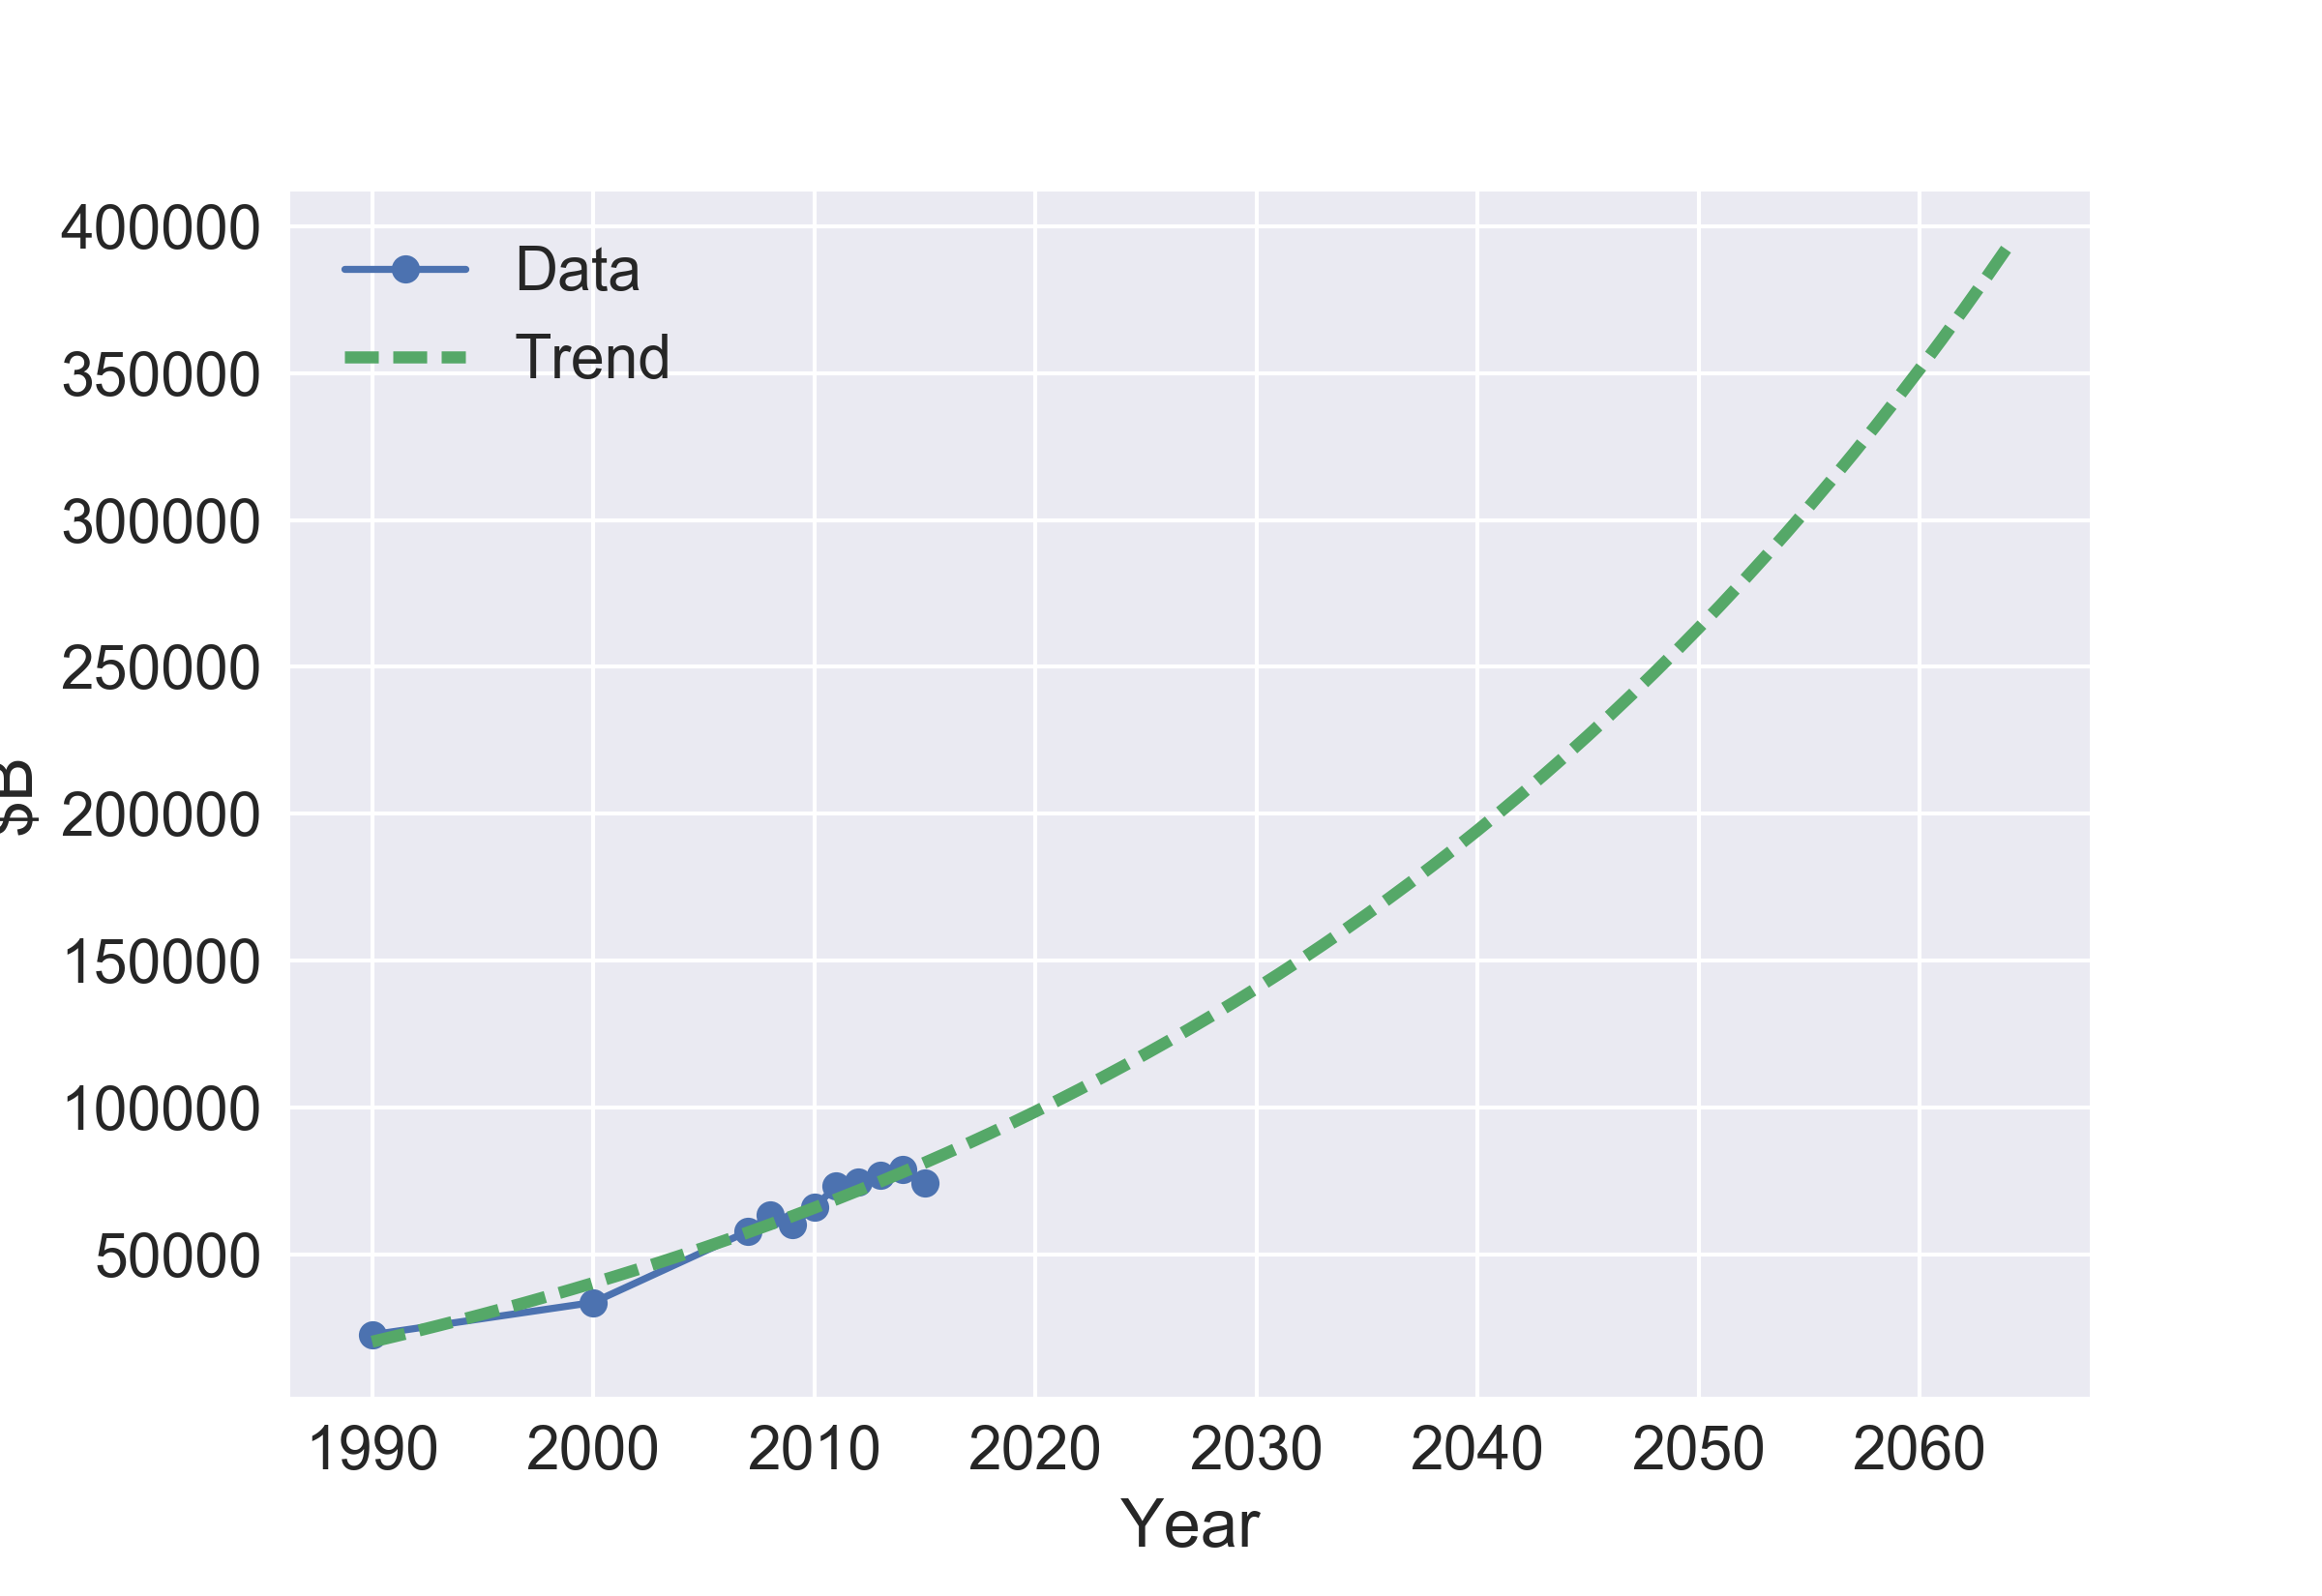
\includegraphics[scale=0.5]{wedge_calculator/GWP.png}
\caption{Projected GWP up to 2064 based on a exponential trend ($ae^{bx}+c$) with data from 1990 to 2015.}
\label{}
\end{figure}

We see that in 2065 the expect GWP is \$40,4307 B, which is around 5.13 x times higher relative to the 2015 levels. If we use an average world growth rate instead (\url{https://en.wikipedia.org/wiki/Gross_world_product}) of 3.2\%, compounded after 50 years this is 4.83 x times the original value. This value can oscillate a lot, between 5 and negative (recent economic recession/crisis), so we will the exponential curve fit for our purposes.

\subsection{Energy and $CO_2$ displacement}

For the next exercises we will be seeing how other forms of electricity can displace energy and $CO_2$ generation, otherwise known as carbon abatement, for this we will assume the new power plant will replace the construction of a mix of coal and gas power plants since these are the most used for electricity generation. If we considered the replacement would come from another source (EV vehicles, biomass, etc), these numbers would change. Currently coal accounts for 40.8\% and gas 21.6\%  of world electricity generation.

Under this mix, for each unit (KWh) of electricity we want to see how much carbon is produced on average. Coal which produces around 1,001 g $CO_2$ per kWh (\url{http://www.nrel.gov/analysis/sustain_lca_coal.html}) and gas produces 470g $CO_2$ per kWh (\url{http://www.nrel.gov/analysis/sustain_lca_ngas.html}). So for one KWh that is generated from our clean energy sources, we will be displacing $1001 \times \frac{40.8}{62.4} + 470 \times \frac{21.6}{62.4} = 817.19\;g\;CO_2$ or $222.66\;g\;C$ per KWh. This is assuming that the alternative energy does not produce C, this is not true, but we will consider it negligible.

For more relevant units, we see that to displace one kg of C we need to generate 4.491 KWh from clean energy sources, or one metric ton of C will require 4491 KWh of energy. Therefore the end-goal of one wedge (1 BMt of C) represents $4491 KWh \times 10^9$ or 4,491 TWh of generated energy.


\subsection{Scenarios}

We can choose how fast to converge on the end-goal of energy generation requirements by considering two scenarios:

\begin{itemize}
\item \textbf{Linear capacity growth (lin g)}: Each year we invest in capacity in a linear fashion, i.g. the first year we build 1 plant, next year we build another plant (now we have 2)...and so on. Each year the cost will ramp up linearly since we are paying energy via LCOE.
\item \textbf{Fixed GWP (f GWP)}: Each year we invest a fixed percentage of GWP, since growth is exponential then we expect to invest a constant amount making the outcome predictable and the amount of money to invest directly tied to the economy. Also we expect installed capacity to growth exponentially. It should be noted this is a direct comparison of a linear growth model, since the accumulative carbon that is abated is different (the area of the wedge). Since climate change is a accumulative problem, one solution might be better than the other.
\end{itemize}


\subsection{Calculations of cost, capacity and GWP}

For the calculations, we can use the capacity factor of a typical plant and the number of hours in a year to estimate the amount of capacity that has to be built via $cap=\frac{4,491 TWh}{8760 h\times {cap}_{factor}}$ at the end of the wedge.

To estimate how much money should be invested to reach the desired energy generation we use a LCOE figure, since multiplying the cost of one KWh and the number of required KWh we can get the cost of abating one ton of C.

LCOE takes into account the overnight capital cost, the lifetime of the plant which factors into the capital recovery factor (CRF) along with the interest rate and the capacity factor. 

To calculate the percentage of GWP that is invested, we just take the cost at a particular year using one energy technology and divide by the GWP at that year.

These calculations are summarized in three plots:
\begin{itemize}
\item \textbf{Global capacity}: Shows how much total global capacity is incrementally installed across time.
\item \textbf{Annual Growth rate}: Plot of the relative growth in capacity from one year to another. Is capacity building slowing down or ramping up?
\item \textbf{GWP cost}: Shows the percentage of GWP that will be invested in one technology. 
\end{itemize}

\section{Solar Power}

\subsection{Assumptions}
\begin{itemize}
\item \textbf{Global Installed Capacity}: 302 GW as of 2015 (\url{https://en.wikipedia.org/wiki/Growth_of_photovoltaics}).
\item \textbf{Lifetime}: 25 to 40 years of useful life. Efficiency drops to 80\% or below after 20 years of operation. The amount of time is mostly going to effect the interest rate and the CRF within the LCOE formula. (\url{http://www.nrel.gov/analysis/tech_footprint.html})
\item \textbf{Capacity Factor}: 20\%, this is using the average capacity factor. In a ideal situation you would build the massive PV infrastructure in a hot desert area. (Transparent Cost Database: \url{http://en.openei.org/apps/TCDB/#blank}, \url{http://www.nrel.gov/analysis/tech_cap_factor.html})
\item \textbf{Overnight Capital cost:} \$ 4.55k median, or as low as \$ 1.5k per installed KW.
\item \textbf{LCOE}: \$55 per MWh  as an average for unsubsidized silicon utility scale PV, taken from Lazard's LCOE anlaysis 2016 (\url{https://www.lazard.com/media/438038/levelized-cost-of-energy-v100.pdf}, page 3).
\end{itemize}

\subsection{Stats}
\begin{itemize}
\tightlist
\item
  LCOE of \$0.0550 per KWh with capacity factor of 0.200
\item
  From an initial capacity of 302.00 GW
\item
  To a 50 year capacity of 2865.36 GW (2563.36 GW more)
\item
  Which means 8.49 x more capacity will be built.

  \begin{itemize}
  \tightlist
  \item
    at 1th year the capacity is 353.27 GW (16.98 \% more from last year)
  \item
    at 50th year the capacity is 2865.36 GW (1.82 \% more from last
    year)
  \end{itemize}
\item
  With linear growth in capacity of 2.00 \%

  \begin{itemize}
  \tightlist
  \item
    at 1th year this is 2.01\% of GWP, or \$1633.09 B
  \item
    at 50th year this is 20.77\% of GWP, or \$81654.55 B
  \end{itemize}
\item
  With fixed GWP investment in 50 years

  \begin{itemize}
  \tightlist
  \item
    at 1th year this is 20.77\% of GWP, or \$16847.99 B
  \item
    at 50th year this is 20.77\% of GWP, or \$81654.55 B
  \end{itemize}
\item
  With exp growth in capacity in 50 years

  \begin{itemize}
  \tightlist
  \item
    at 1th year the capacity is 852.49 GW (2.60 \% more from last year)
  \item
    at 50th year the capacity is 2865.36 GW (2.53 \% more from last
    year)
  \end{itemize}
\end{itemize}

\subsection{Results}

\colorbox{harvardcrimson!20}{ \textbf{a)}  } 20.77\% of GWP by 2050


\colorbox{harvardcrimson!20}{ \textbf{b)} } The fixed value of GWP would also be 20.77\% since the end goal of reduction is the same, thou the accumulative C reduction across would be different. The ratio of GPW from now to to the future is 5.13. 

\colorbox{harvardcrimson!20}{ \textbf{c)} }  For the first year, linear growth is 22.39 \%

\colorbox{harvardcrimson!20}{ \textbf{d)} } We can compare with 2015 which saw a growth rate of 29\%. Our estimates are below, but close!. (\url{https://en.wikipedia.org/wiki/Growth_of_photovoltaics}).

\section{Wind}

\subsection{Assumptions}
\begin{itemize}
\item \textbf{Global Installed Capacity}: 432 GW as of 2015 (\url{https://en.wikipedia.org/wiki/Wind_power_by_country}).
\item \textbf{Lifetime}: 20 years of useful life. After that the wind turbine requires extensive refactoring. A real simulation would take repair costs in to consideration in order to maximize profit from existing infrastructure.(\url{http://www.nrel.gov/analysis/tech_footprint.html})
\item \textbf{Capacity Factor}: 38\%, this is using the average capacity factor. (Transparent Cost Database: \url{http://en.openei.org/apps/TCDB/#blank}, \url{http://www.nrel.gov/analysis/tech_cap_factor.html})
\item \textbf{Overnight Capital cost:} \$ 2.03k median per installed KW. (Transparent Cost Database: \url{http://en.openei.org/apps/TCDB/#blank})
\item \textbf{LCOE}: \$48 per MWh  as utility scale onshore wind turbines, taken from Lazard's LCOE anlaysis 2016 (\url{https://www.lazard.com/media/438038/levelized-cost-of-energy-v100.pdf}, page 3).
\end{itemize}

\subsection{Stats}
\begin{itemize}
\tightlist
\item
  LCOE of \$0.0480 per KWh with capacity factor of 0.200
\item
  From an initial capacity of 432.00 GW
\item
  To a 50 year capacity of 2995.36 GW (2563.36 GW more)
\item
  Which means 5.93 x more capacity will be built.

  \begin{itemize}
  \tightlist
  \item
    at 1th year the capacity is 483.27 GW (11.87 \% more from last year)
  \item
    at 50th year the capacity is 2995.36 GW (1.74 \% more from last
    year)
  \end{itemize}
\item
  With linear growth in capacity of 2.00 \%

  \begin{itemize}
  \tightlist
  \item
    at 1th year this is 2.31\% of GWP, or \$1871.25 B
  \item
    at 50th year this is 23.80\% of GWP, or \$93562.50 B
  \end{itemize}
\item
  With fixed GWP investment in 50 years

  \begin{itemize}
  \tightlist
  \item
    at 1th year this is 23.80\% of GWP, or \$19304.98 B
  \item
    at 50th year this is 23.80\% of GWP, or \$93562.50 B
  \end{itemize}
\item
  With exp growth in capacity in 50 years

  \begin{itemize}
  \tightlist
  \item
    at 1th year the capacity is 982.49 GW (2.25 \% more from last year)
  \item
    at 50th year the capacity is 2995.36 GW (2.42 \% more from last
    year)
  \end{itemize}
\end{itemize}
\subsection{Answers}


\colorbox{harvardcrimson!20}{ \textbf{a)}  } 23.80\% of GWP by 2050


\colorbox{harvardcrimson!20}{ \textbf{b)} } The fixed value of GWP would also be 23.80\% since the end goal of reduction is the same, thou the accumulative C reduction across would be different. The ratio of GPW from now to to the future is 5.13. 

\colorbox{harvardcrimson!20}{ \textbf{c)} }  For the first year, linear growth is 11.87 \%. 

\colorbox{harvardcrimson!20}{ \textbf{d)} } We can compare with 2015 which saw a growth rate of 15.9\%. Our estimates are below, but close!. (\url{https://en.wikipedia.org/wiki/Wind_power_by_country})


\section{Nuclear}

\subsection{Assumptions}
\begin{itemize}
\item \textbf{Global Installed Capacity}: 392 GW as of 2015 (\url{https://en.wikipedia.org/wiki/Nuclear_power_by_country}).
\item \textbf{Lifetime}: 40-60 years, after which it will have to be decommissioned.(\url{https://phys.org/news/2011-05-nuclear-power-world-energy.html})
\item \textbf{Capacity Factor}: 90\%, this is using the median capacity factor. (Transparent Cost Database: \url{http://en.openei.org/apps/TCDB/#blank}, \url{http://www.nrel.gov/analysis/tech_cap_factor.html})
\item \textbf{Overnight Capital cost:} \$ 5.30k median per installed KW. (Transparent Cost Database: \url{http://en.openei.org/apps/TCDB/#blank})
\item \textbf{LCOE}: \$116.5 per MWh  as an average within the range of variance, taken from Lazard's LCOE anlaysis 2016 (\url{https://www.lazard.com/media/438038/levelized-cost-of-energy-v100.pdf}, page 3).
\end{itemize}

\subsection{Stats}

\begin{itemize}
\tightlist
\item
  LCOE of \$0.1165 per KWh with capacity factor of 0.900
\item
  From an initial capacity of 392.00 GW
\item
  To a 50 year capacity of 961.63 GW (569.63 GW more)
\item
  Which means 1.45 x more capacity will be built.

  \begin{itemize}
  \tightlist
  \item
    at 1th year the capacity is 403.39 GW (2.91 \% more from last year)
  \item
    at 50th year the capacity is 961.63 GW (1.20 \% more from last year)
  \end{itemize}
\item
  With linear growth in capacity of 2.00 \%

  \begin{itemize}
  \tightlist
  \item
    at 1th year this is 0.95\% of GWP, or \$770.99 B
  \item
    at 50th year this is 9.80\% of GWP, or \$38549.36 B
  \end{itemize}
\item
  With fixed GWP investment in 50 years

  \begin{itemize}
  \tightlist
  \item
    at 1th year this is 9.80\% of GWP, or \$7953.98 B
  \item
    at 50th year this is 9.80\% of GWP, or \$38549.36 B
  \end{itemize}
\item
  With exp growth in capacity in 50 years

  \begin{itemize}
  \tightlist
  \item
    at 1th year the capacity is 514.33 GW (0.94 \% more from last year)
  \item
    at 50th year the capacity is 961.63 GW (1.66 \% more from last year)
  \end{itemize}
\end{itemize}

\subsection{Answers}

\colorbox{harvardcrimson!20}{ \textbf{a)}  } 9.80\% of GWP by 2050


\colorbox{harvardcrimson!20}{ \textbf{b)} } The fixed value of GWP would also be 9.80\% since the end goal of reduction is the same, thou the accumulative C reduction across would be different. The ratio of GPW from now to to the future is 5.13. 

\colorbox{harvardcrimson!20}{ \textbf{c)} }  For the first year, linear growth is 2.91 \%. 

\colorbox{harvardcrimson!20}{ \textbf{d)} } We can compare with 2015 which saw a growth rate of 17\%. Our estimates are WAY below! (in a good way). (\url{https://en.wikipedia.org/wiki/Wind_power_by_country})


(\url{https://en.wikipedia.org/wiki/Nuclear_power_by_country}).

\section{Final results}

\begin{figure}[htp]
\centering
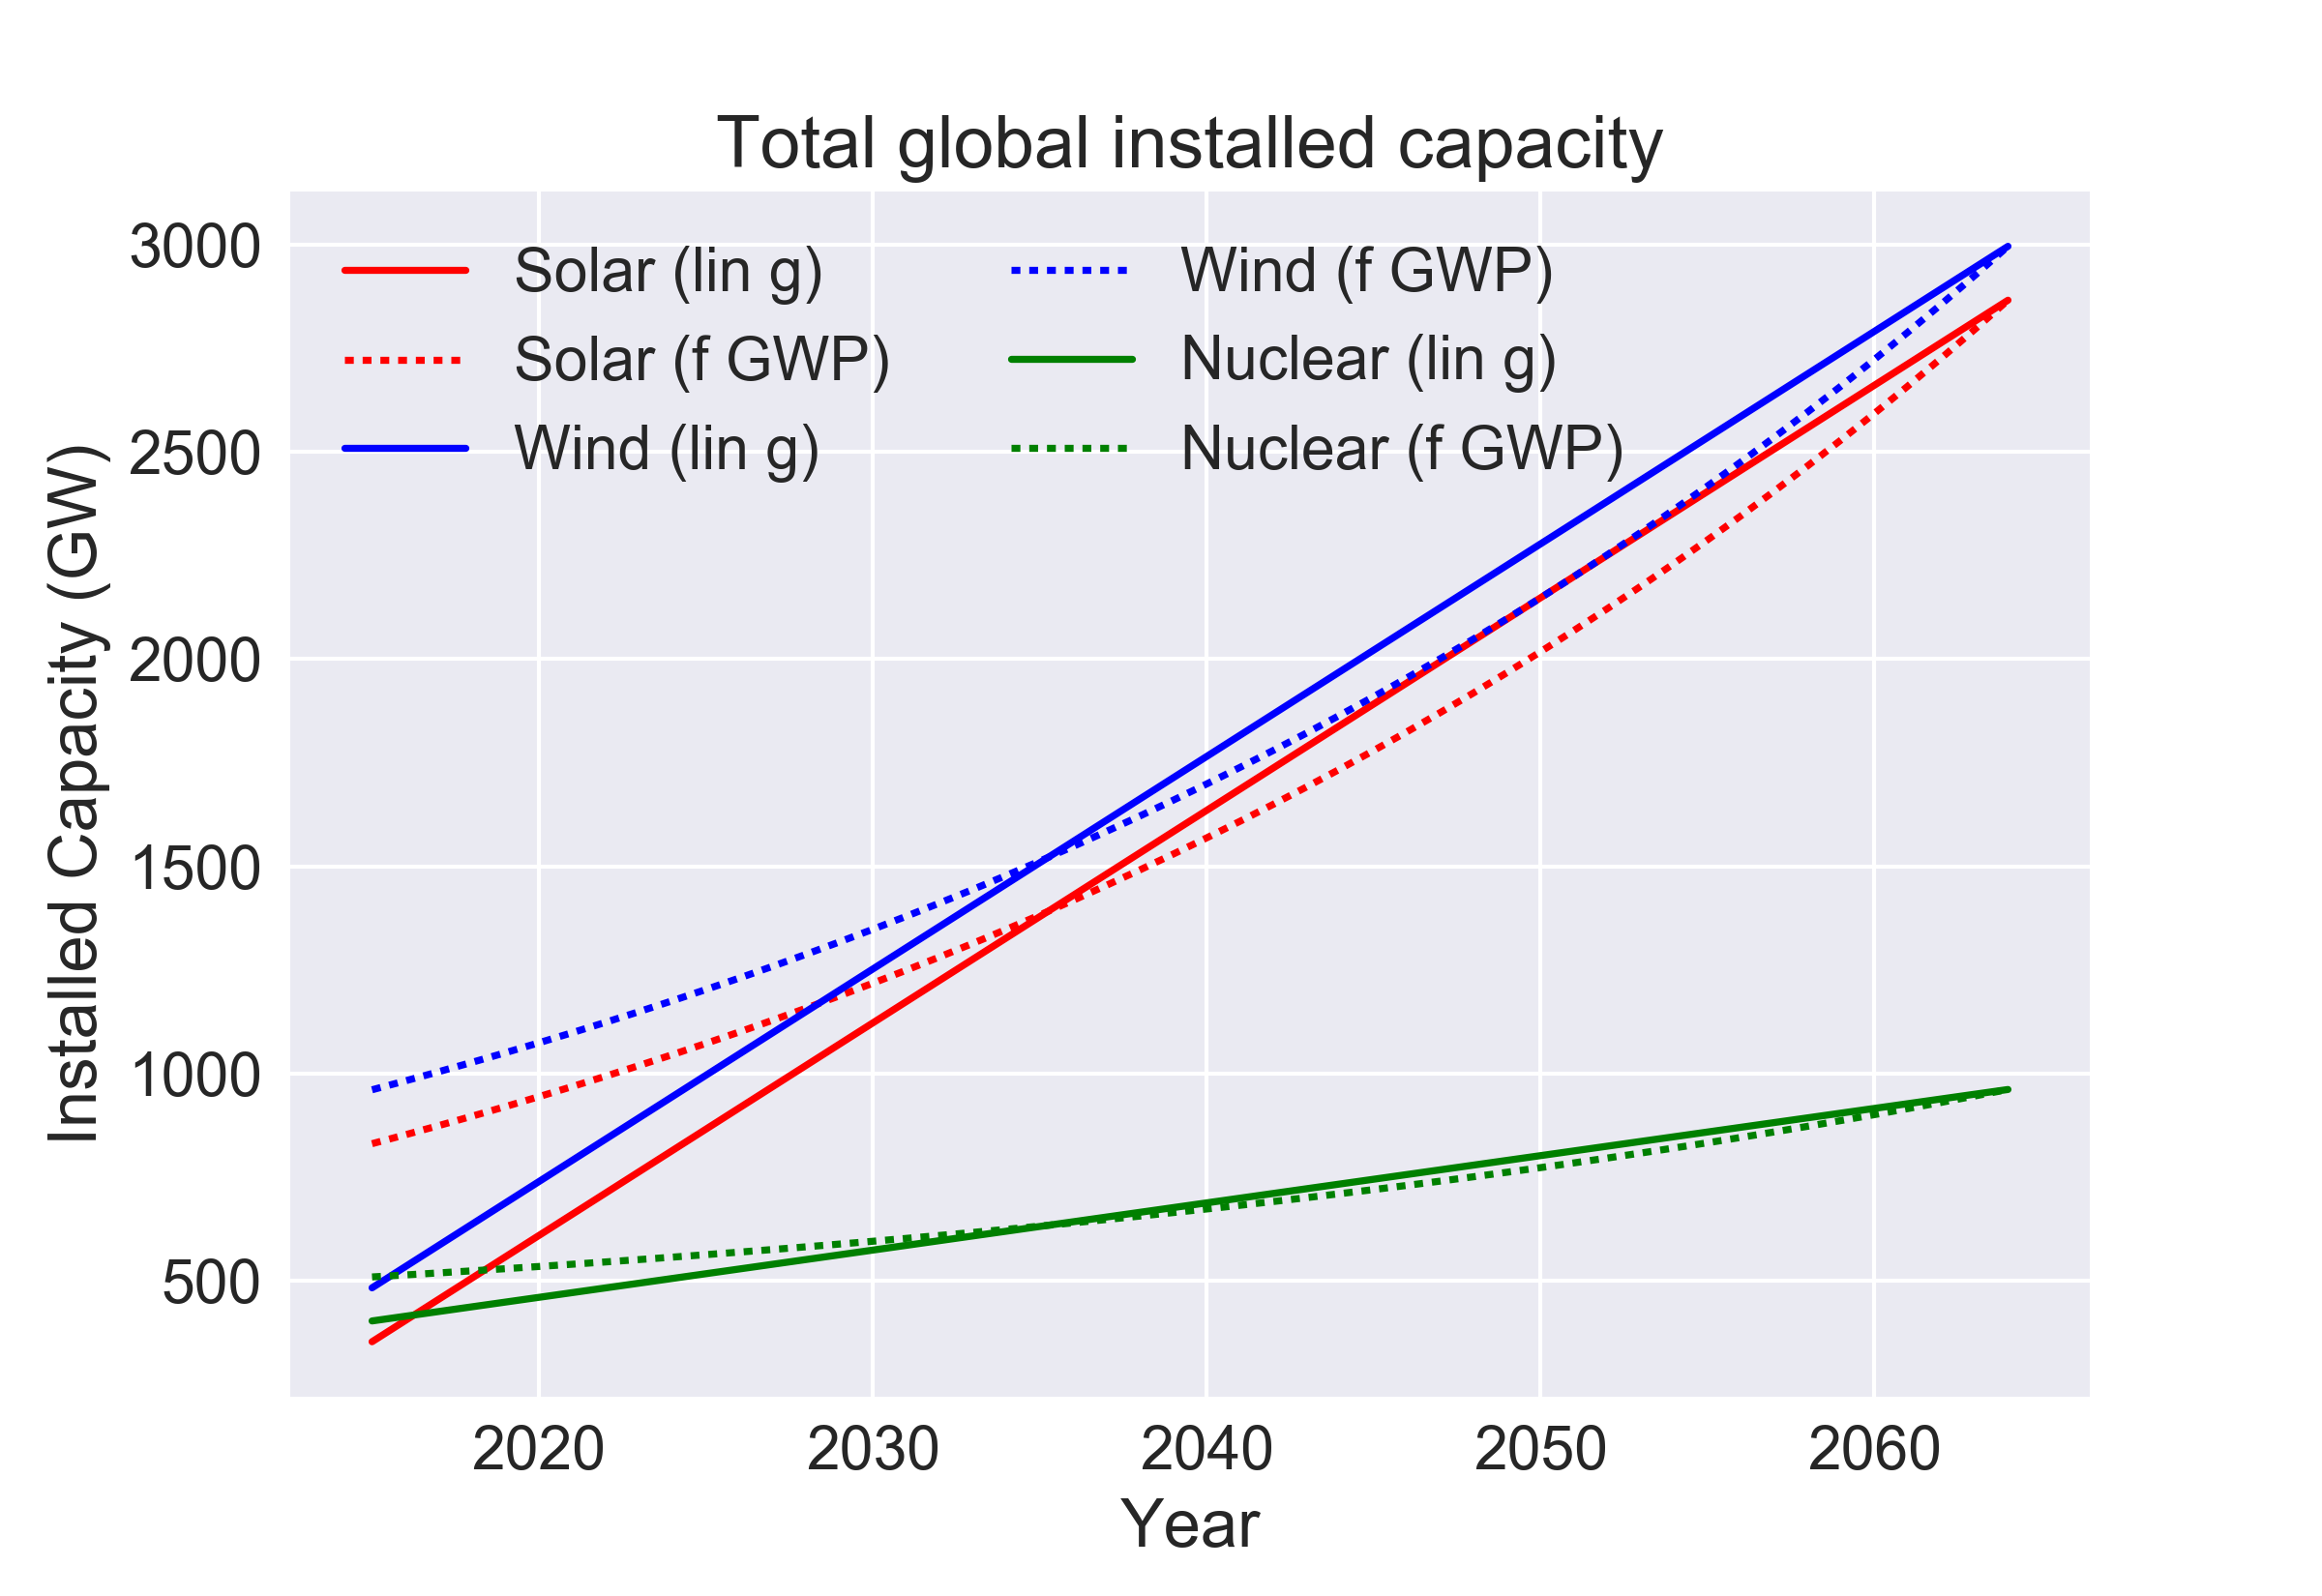
\includegraphics[scale=0.6]{wedge_calculator/cap_installed.png}
\caption{Global capacity}
\label{}
\end{figure}

\begin{figure}[htp]
\centering
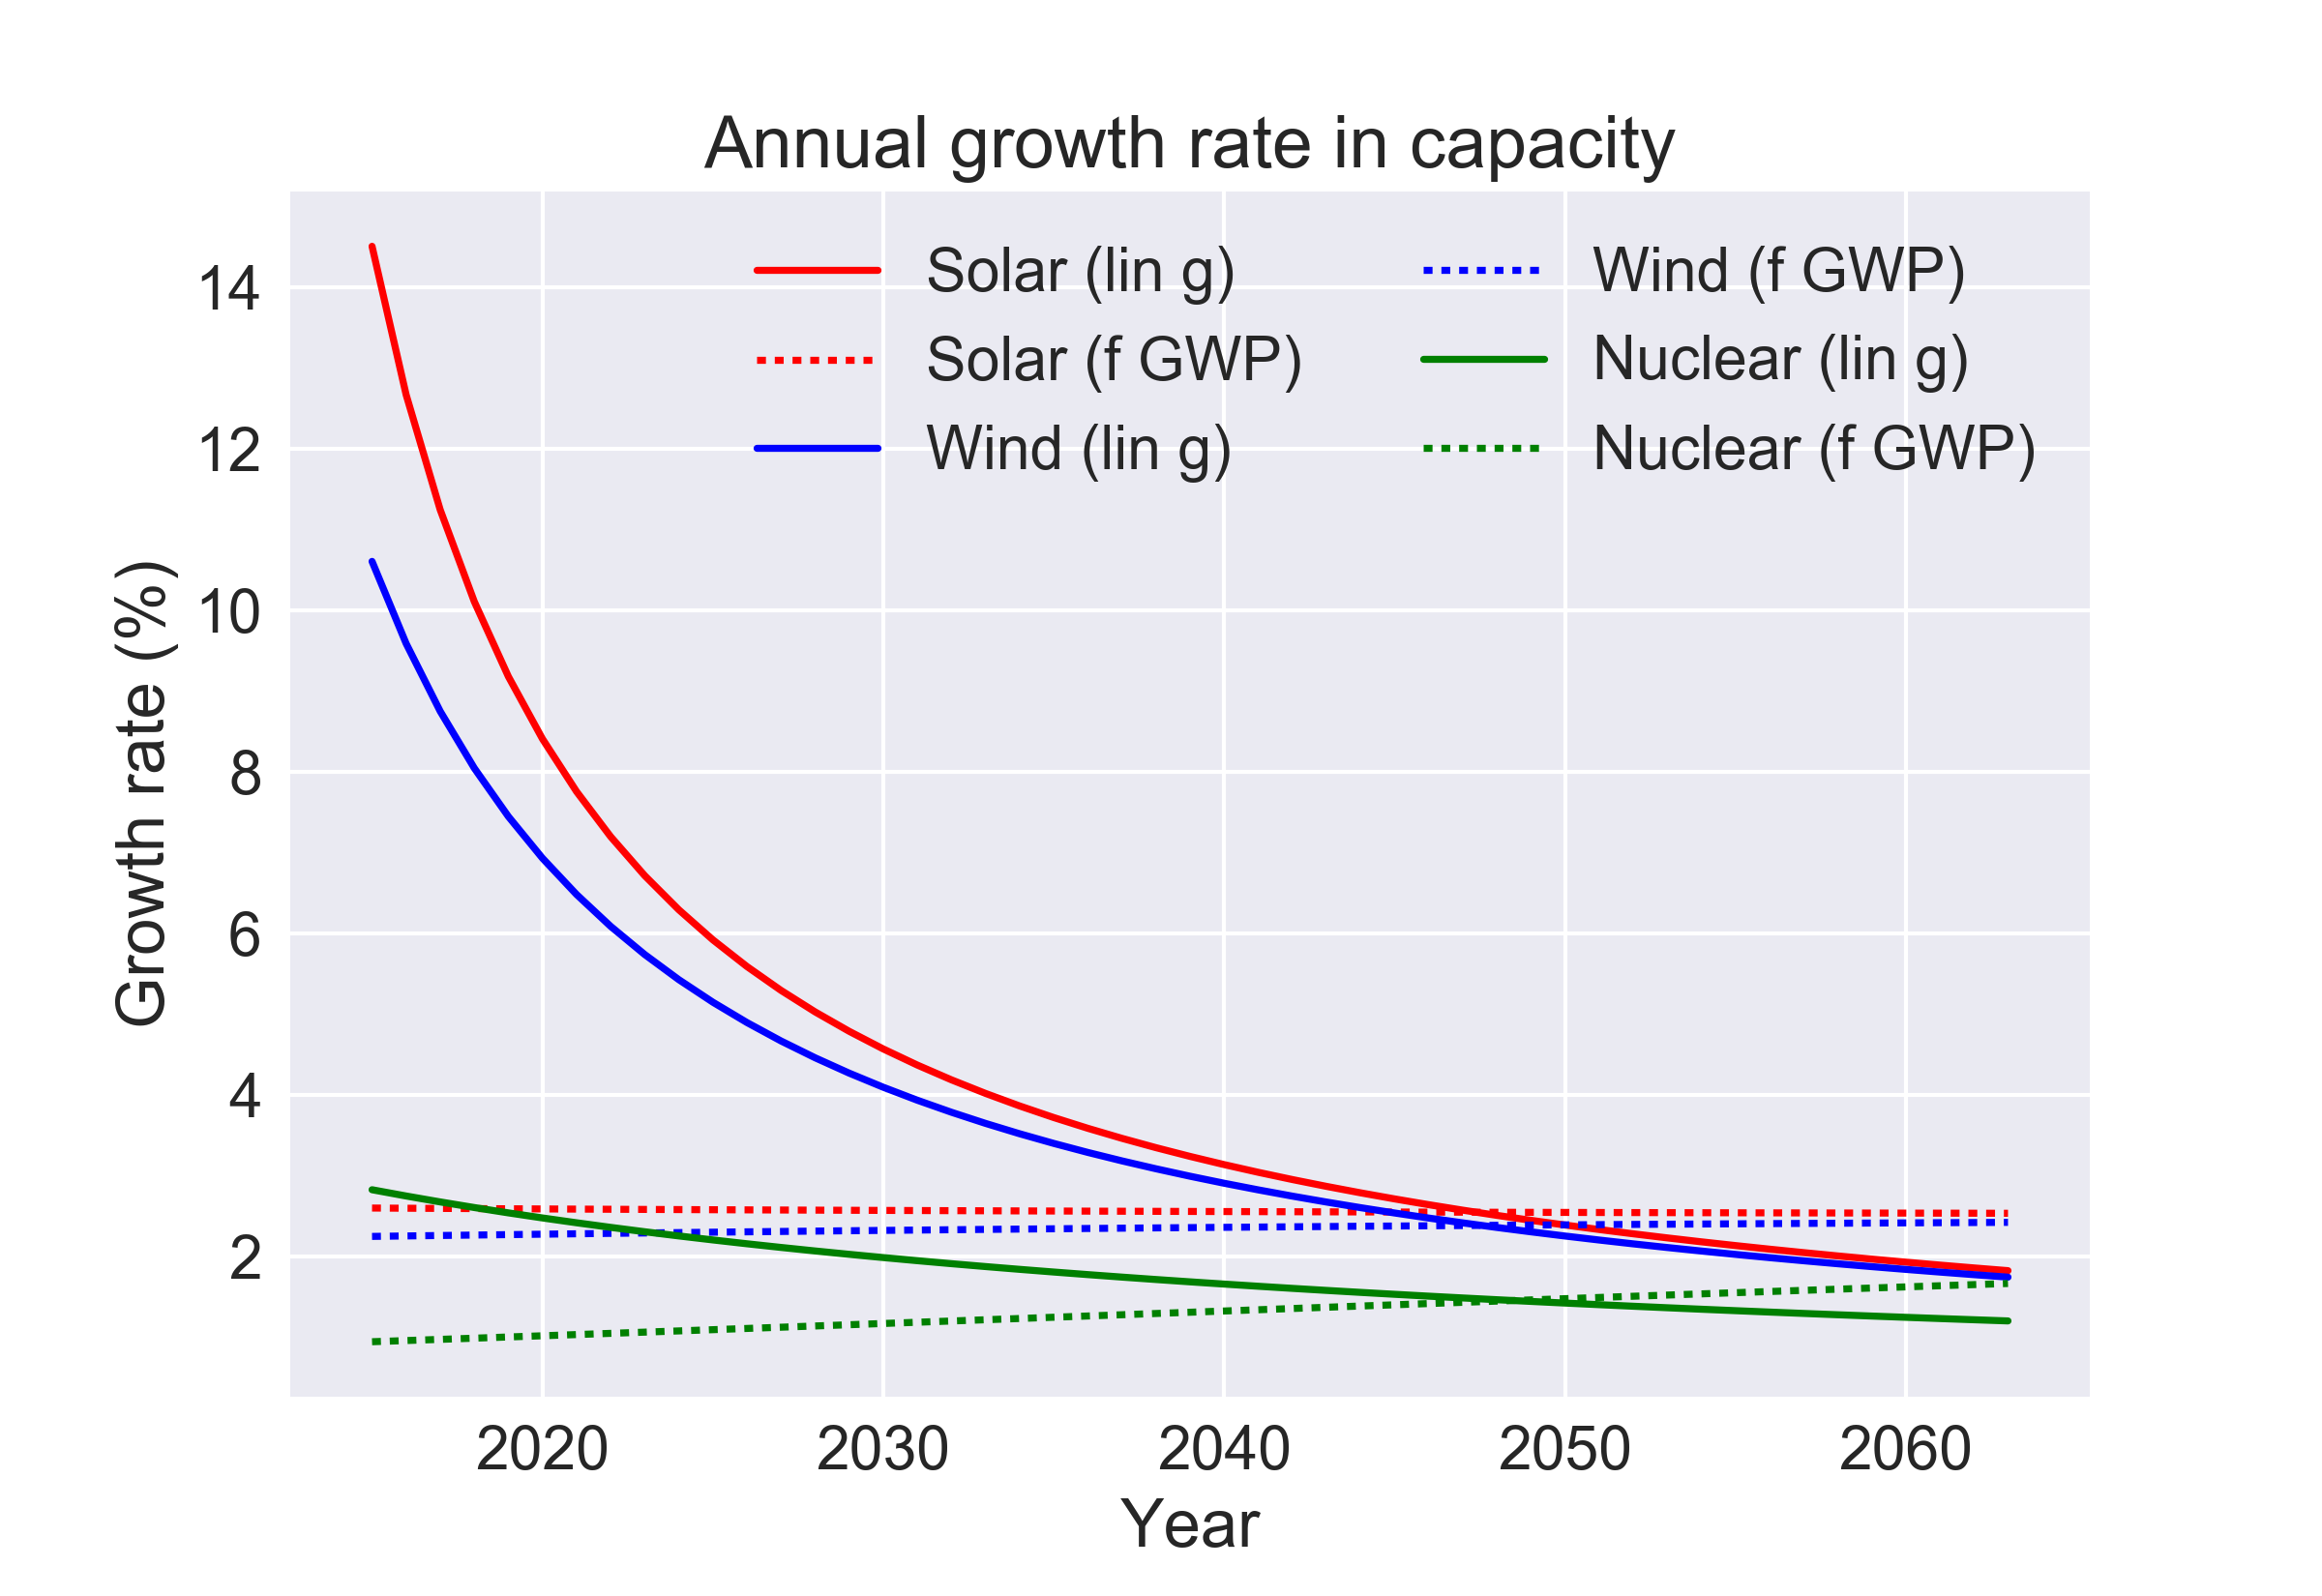
\includegraphics[scale=0.6]{wedge_calculator/cap_growth.png}
\caption{Annual Growth rate}
\label{}
\end{figure}

\begin{figure}[htp]
\centering
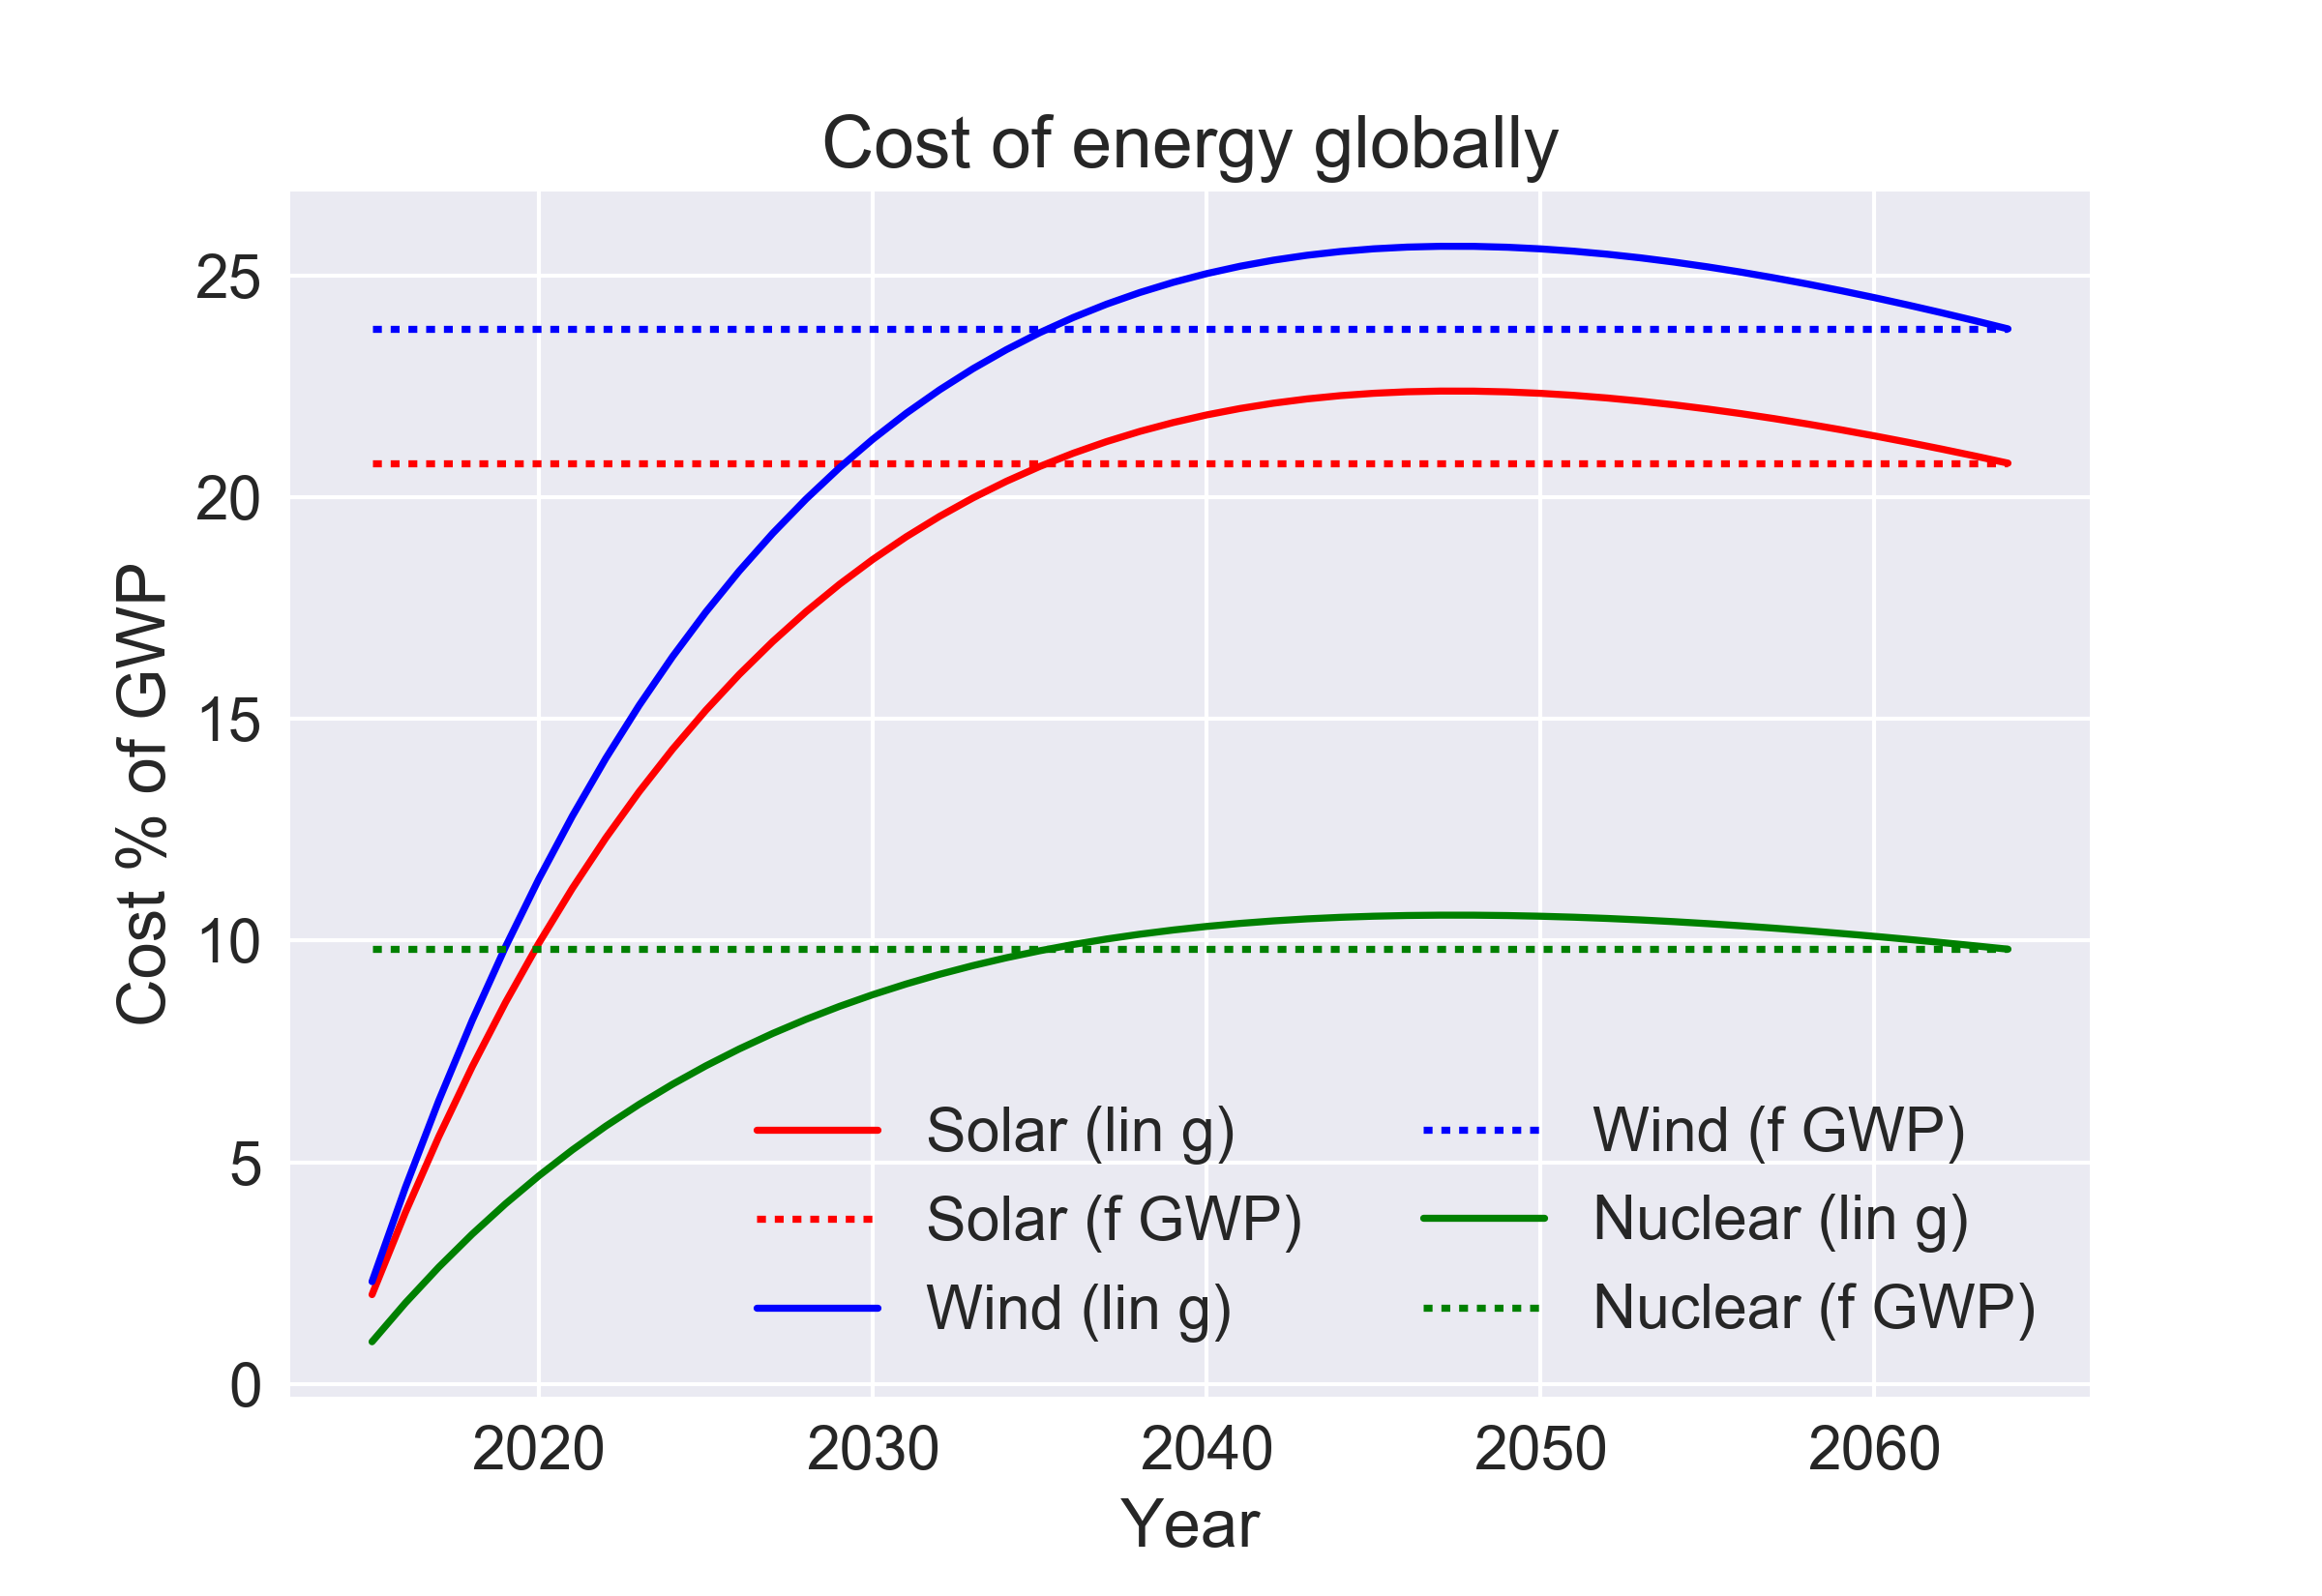
\includegraphics[scale=0.6]{wedge_calculator/GWP_cost.png}
\caption{GWP cost}
\label{}
\end{figure}


\end{document}
